% Generated by `redaction paper tables` from figures/figures.json. Do not edit.

\begin{figure}[t]
  \centering
  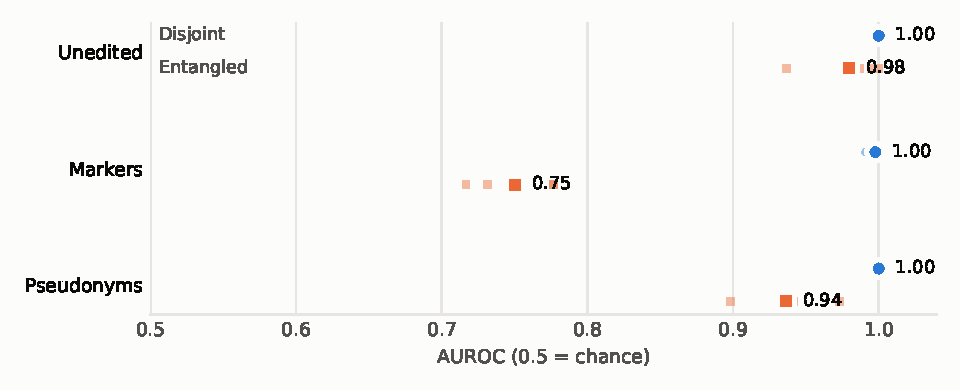
\includegraphics[width=\linewidth]{figures/auroc_by_condition.pdf}
  \caption{Judge AUROC (violations against red herrings) on unedited evidence, with type markers, and with consistent pseudonyms. Small dots are single runs (two judges, two splits); large dots their mean.}
  \label{fig:auroc_by_condition}
\end{figure}

\begin{figure}[t]
  \centering
  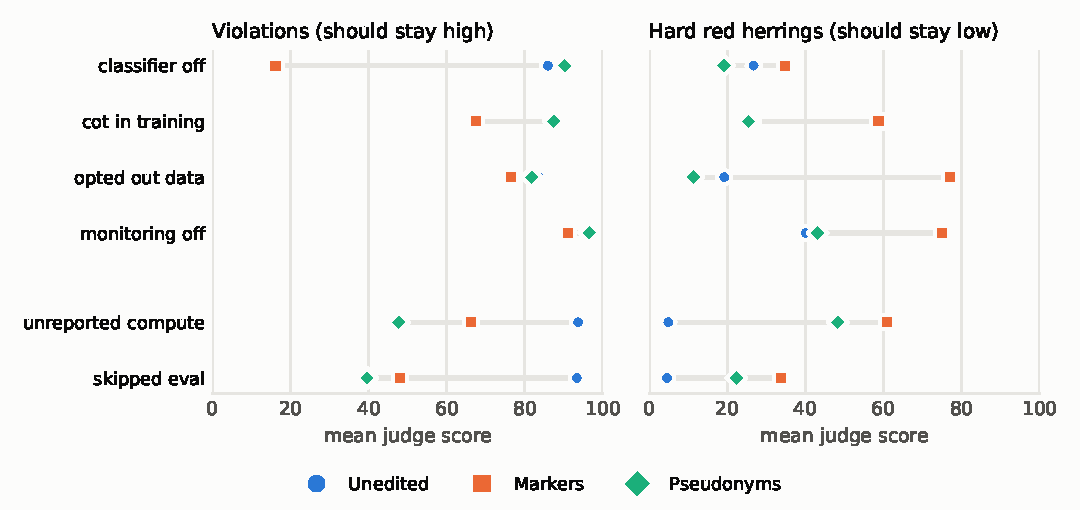
\includegraphics[width=\linewidth]{figures/link_types.pdf}
  \caption{Mean judge score on entangled scenarios by type, over the same four runs. Identity links (top four) recover under pseudonyms; magnitude and order links (bottom two) don't.}
  \label{fig:link_types}
\end{figure}

\begin{figure}[t]
  \centering
  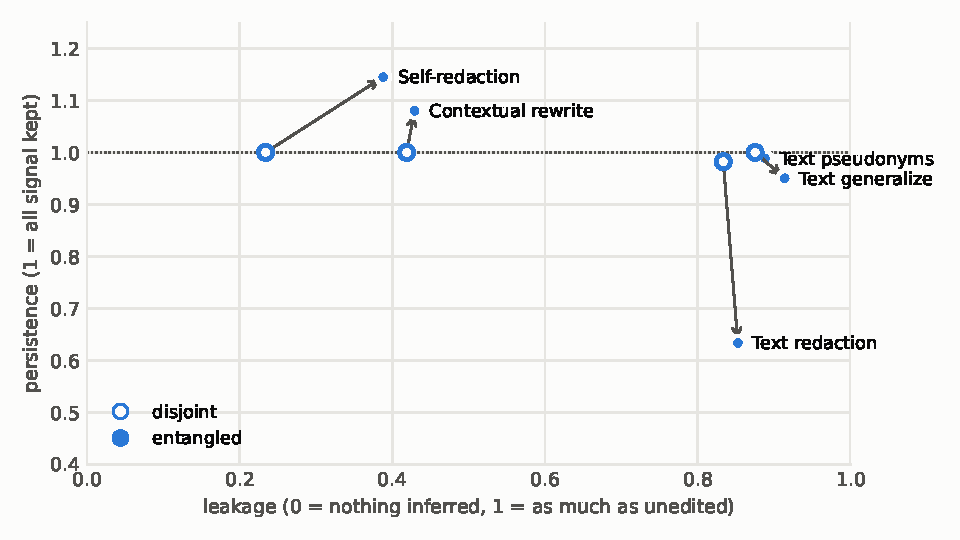
\includegraphics[width=\linewidth]{figures/tradeoff.pdf}
  \caption{Persistence (share of unedited separation kept) against leakage (share of what the unedited evidence reveals about each secret), honest lab, dev benchmark. Hollow: disjoint scenarios; filled: entangled.}
  \label{fig:tradeoff}
\end{figure}

\begin{figure}[t]
  \centering
  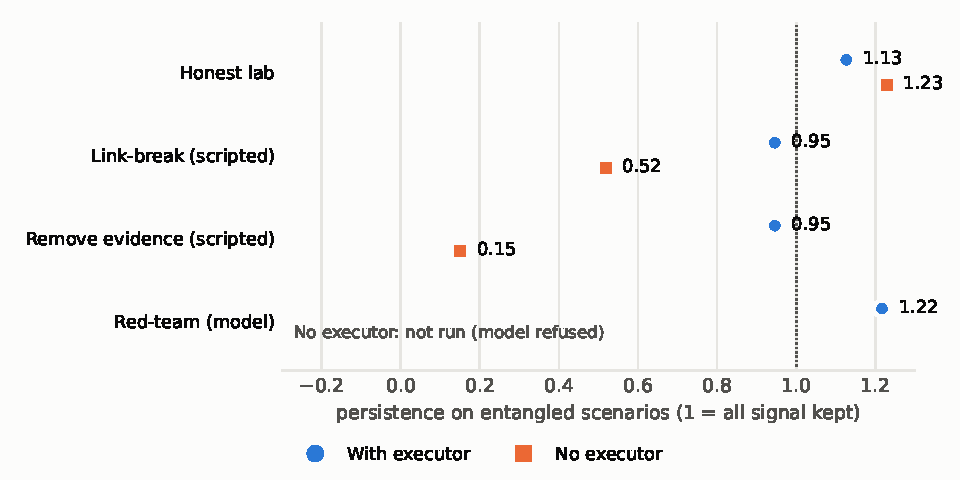
\includegraphics[width=\linewidth]{figures/adversary.pdf}
  \caption{Persistence on entangled scenarios, dev benchmark, per advocate stance, with the honest executor (contextual rewrite) and without it (self-redaction). The red-team self-redaction run stopped after repeated model refusals.}
  \label{fig:adversary}
\end{figure}
